\subsection{Study area}\label{subsec:study-area}

The Ramis River basin is located in the high-Andean Altiplano of
southern Peru and drains towards Lake Titicaca. The basin is therefore
part of a closed lacustrine system in which river inflow, precipitation
and evaporation exert strong control on lake-level variability
\citep{cross2001late,condom2004transient,lima2025modeling}. Previous
regional studies show that the hydrology of the Titicaca system is
controlled mainly by rainfall and evapotranspiration variability,
whereas snowmelt, ice melt and net irrigation withdrawals have a
secondary role at the lake-basin scale \citep{lima2025modeling}. This
regional behaviour makes the Ramis basin a relevant test case for a
rainfall--runoff modelling design that combines process-based memory,
stochastic forcing and machine-learning correction.

The basin is characterized by high elevation, sparse hydroclimatic
monitoring and a strongly seasonal precipitation regime. Rainfall is
concentrated during the austral summer wet season, while the dry season
is associated with prolonged recession and low-flow persistence
\citep{condom2004transient,nauditt2017conceptual,lima2025modeling}.
Such hydroclimatic asymmetry is challenging for lumped conceptual
models because a single storage response may be unable to represent both
wet-season peaks and dry-season baseflow. It is also challenging for
purely data-driven models, which may learn strong seasonal correlations
without representing the storage mechanisms that maintain discharge
between rainfall events \citep{van2013influence,lees2021benchmarking}.
Daily discharge observations used in this study correspond to the
Puente Ramis gauging station operated by SENAMHI-Peru.

Figure~\ref{fig:study-area} provides the geographical frame of the
analysis. The delineated catchment, drainage network and model outlet
identify the spatial support over which gridded meteorological products
were aggregated before being used in the lumped rainfall--runoff model.
This step is essential because the model is evaluated at daily time step
and catchment scale; therefore, the consistency between the outlet,
catchment boundary, drainage network and meteorological forcing domain
directly defines the hydrological unit being simulated.

\begin{figure*}[t]
\centering
\IfFileExists{figures/study_area_ramis.png}{%
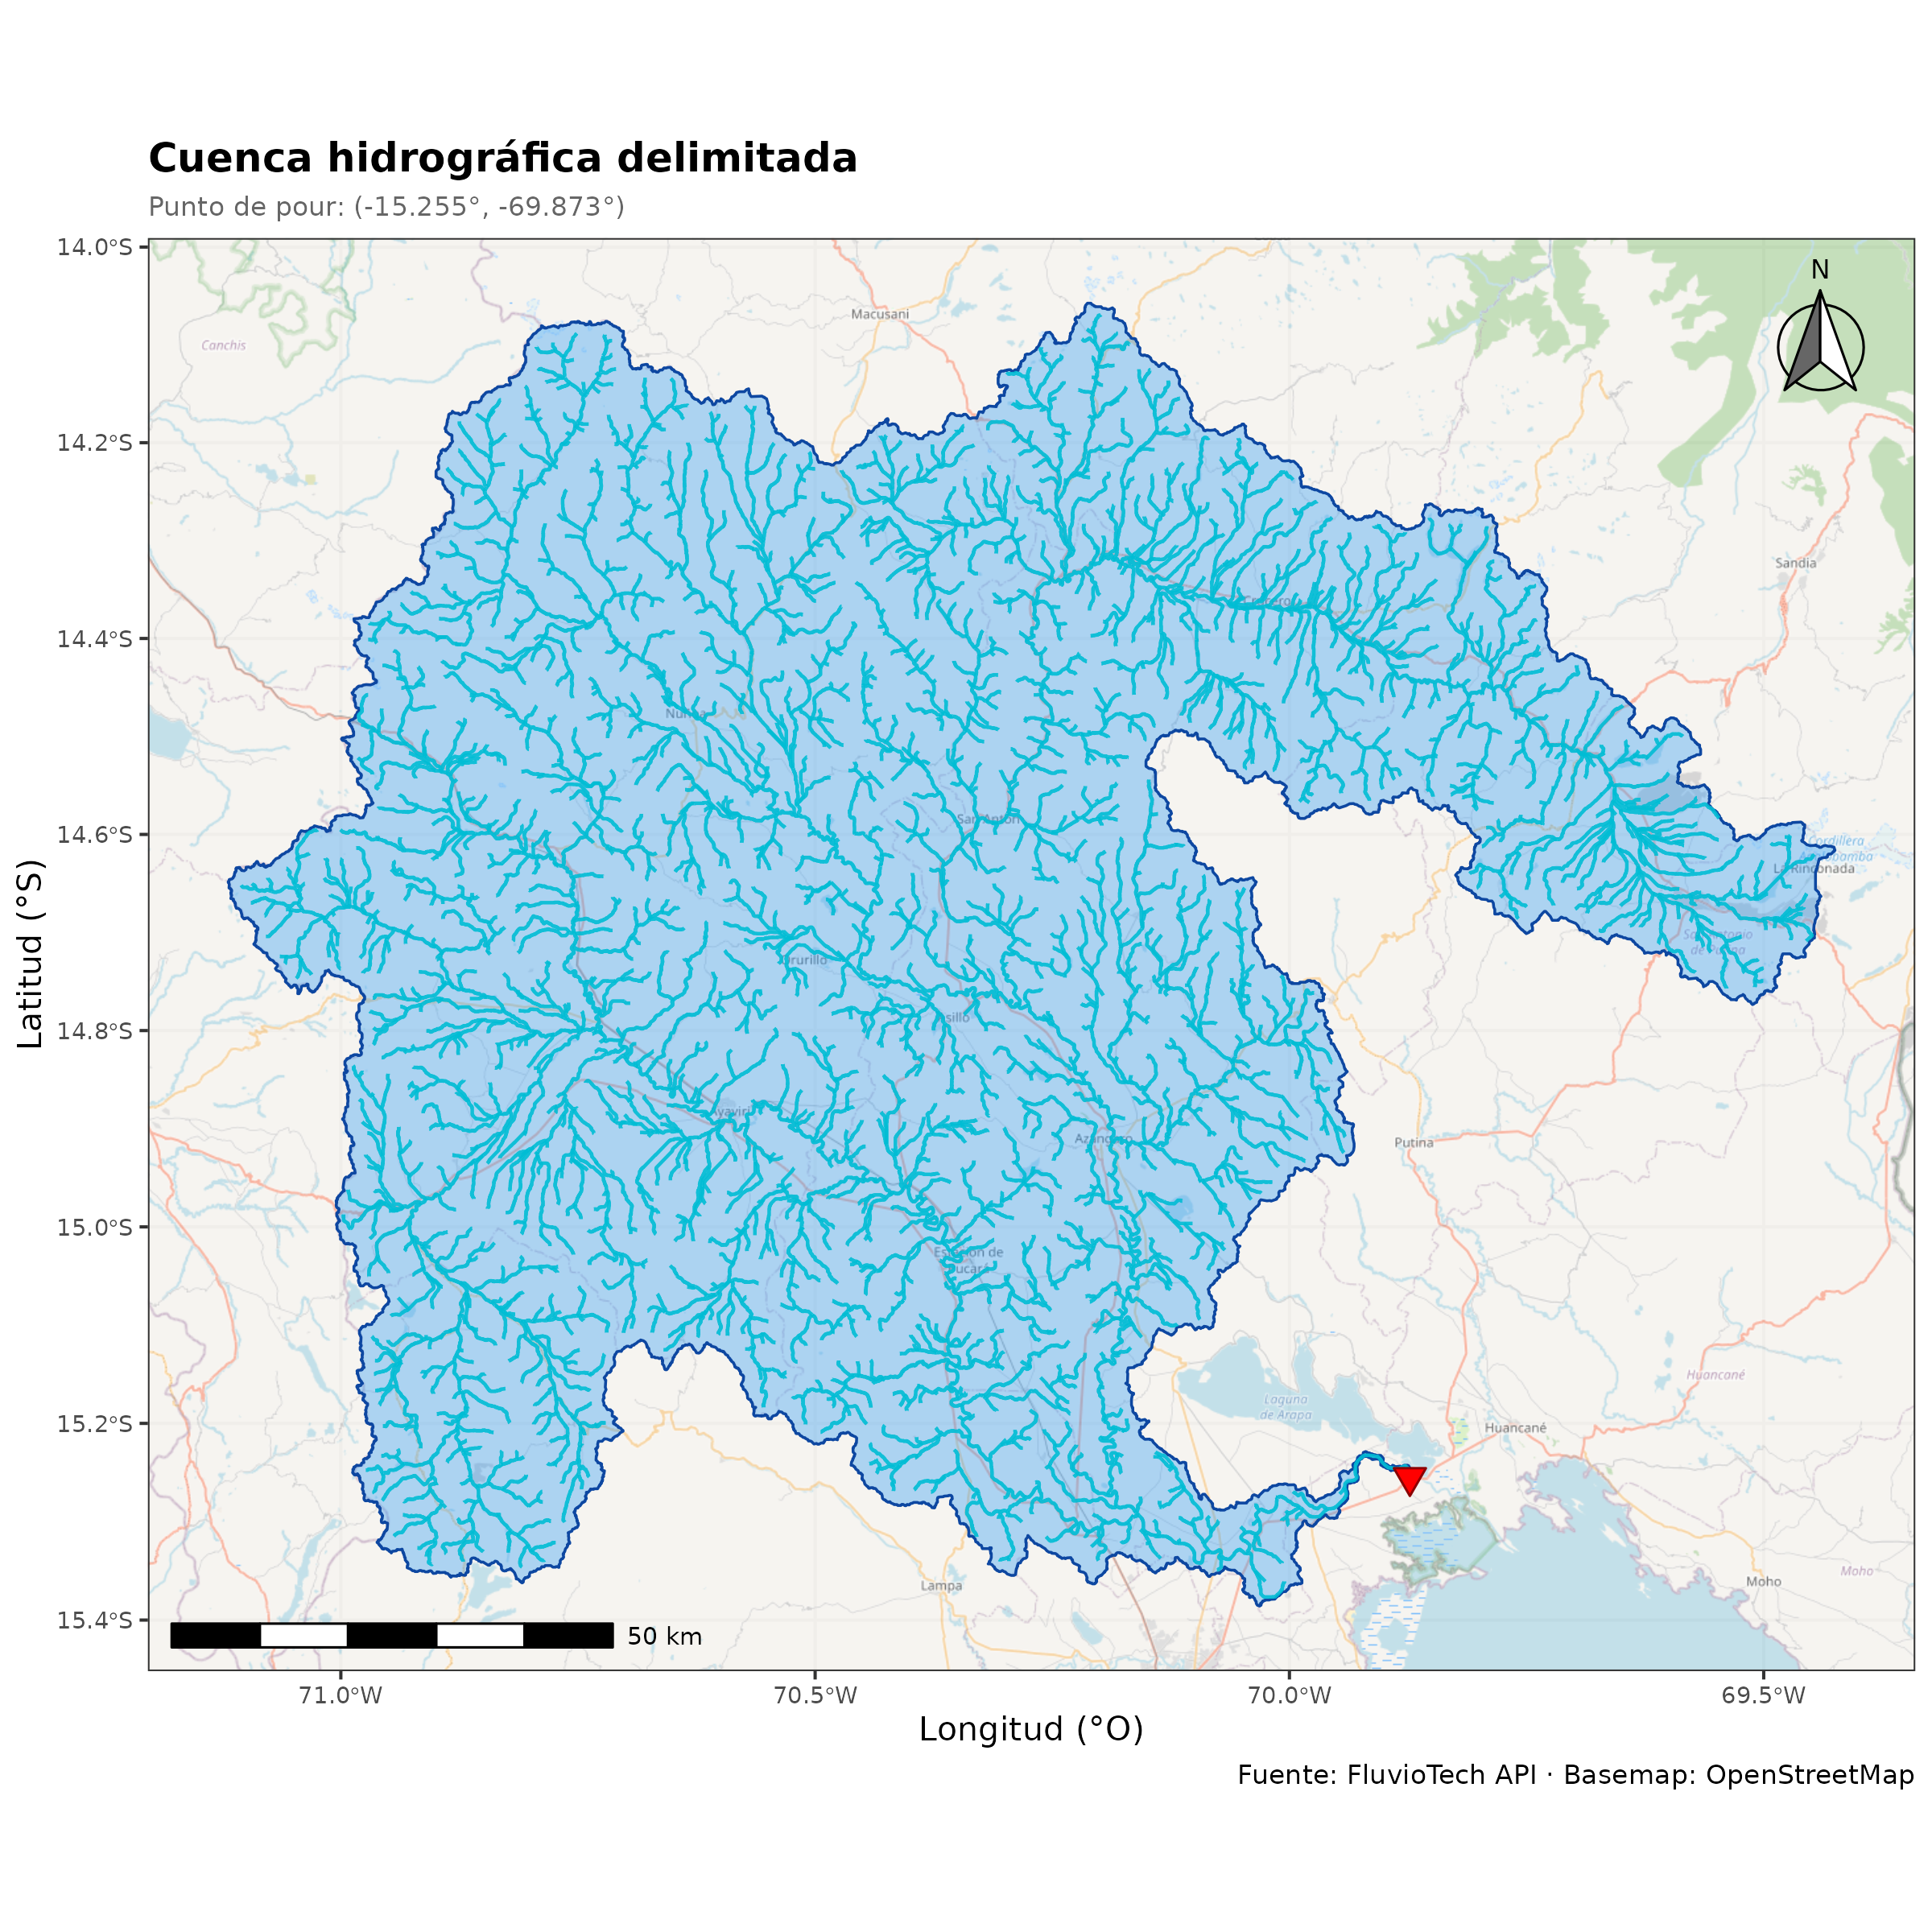
\includegraphics[width=0.92\textwidth]{figures/study_area_ramis.png}%
}{%
\fbox{\parbox[c][0.32\textheight][c]{0.90\textwidth}{\centering
Placeholder for the final study-area map. Replace this box with
\texttt{figures/study\_area\_ramis.png} before submission.}}%
}
\caption{Geographical setting of the Ramis River basin in the
high-Andean Altiplano of southern Peru. The delineated catchment drains
towards Lake Titicaca; the drainage network indicates the main flow
paths represented at catchment scale, and the red marker denotes the
model outlet or pour point used for basin delineation
(15.2550$^{\circ}$S, 69.8730$^{\circ}$W). The map defines the spatial
support used to aggregate gridded precipitation from PISCOp v3.0 and
minimum and maximum air temperature from PISCOt v1.2 into daily
catchment-scale forcings for the lumped rainfall--runoff experiments.}
\label{fig:study-area}
\end{figure*}

%% [AUTHOR ACTION BEFORE SUBMISSION]
%% Insert the official gauged drainage area, station coordinates, gauge
%% elevation and complete record period from SENAMHI/ANA metadata. These
%% details were not included in the materials available for this phase
%% and should not be inferred.

\subsection{Hydro-meteorological data and temporal protocol}
\label{subsec:data-protocol}

The modelling unit is a daily catchment-scale hydro-meteorological
record composed of precipitation ($P_t$), minimum and maximum air
temperature ($T_{\min,t}$ and $T_{\max,t}$), potential
or reference evapotranspiration ($PET_t$) and observed streamflow
($Q^{obs}_t$). Daily precipitation was obtained from the PISCOp v3.0
gridded rainfall product. PISCOp v3.0 is used here as the updated 2026
release of the PISCO precipitation product family; the published
construction of the PISCOp v2.1 rainfall dataset is documented by
\citet{aybar2020construction}. This citation is used to document the
PISCO rainfall dataset family and its gridded-data construction
principles, whereas the specific precipitation input used in this study
corresponds to version~3.0.

Daily minimum and maximum air temperature were obtained from PISCOt
v1.2, a high-resolution gridded daily temperature product for Peru
\citep{huerta2023high}. Precipitation and temperature grids were
spatially aggregated over the delineated Ramis catchment
(Fig.~\ref{fig:study-area}) to obtain basin-mean daily forcing series
for the lumped model. Observed streamflow was taken from the Puente
Ramis gauging station operated by SENAMHI-Peru. All forcing and
discharge series were then aligned at daily time step before model
calibration, ML training and validation.

Potential evapotranspiration was estimated from the PISCOt v1.2
minimum and maximum temperature series using the Hargreaves--Samani
temperature-based formulation \citep{hargreaves1985reference}:
\begin{equation}
PET_t = 0.0023\,R_{a,t}\,(T_{mean,t}+17.8)
        \sqrt{\max(T_{\max,t}-T_{\min,t},0)},
\label{eq:hargreaves-samani}
\end{equation}
where $T_{mean,t}=(T_{\max,t}+T_{\min,t})/2$ and $R_{a,t}$ is
extraterrestrial radiation expressed as equivalent evaporation depth.
With this convention, $PET_t$ is expressed in mm~d$^{-1}$. The
non-negative thermal-amplitude term avoids numerical artefacts if the
processed gridded temperature series contain equal or nearly equal
minimum and maximum values.

The rainfall--runoff core uses an effective precipitation input defined
as
\begin{equation}
P^{eff}_t = \max(P_t - PET_t,\;0),
\label{eq:peff}
\end{equation}
which provides a non-negative approximation of the water available for
runoff generation after atmospheric demand has been accounted for.

All experiments follow the same chronological split. Model calibration
and ML training use data from 8~September~1991 to 31~December~2008,
whereas validation uses data from 8~January~2009 to 31~December~2020.
The final comparative assessment is computed over the common validation
intersection of all experiments, comprising $n=4367$ daily samples. This
common-window design prevents unequal evaluation support across
physical, ML and hybrid configurations and is especially important for
experiments that require lagged predictors or sequence construction.

Temporal leakage was controlled at four levels. First, lagged predictors
were constructed only from present or past information. Second,
sequence samples were generated independently within the training and
validation partitions. Third, scalers and transformations used by ML
models were fitted exclusively on training data and then applied to
validation data. Fourth, flow-regime thresholds used for diagnostic
stratification were estimated from training observations only. These
controls follow the broader hydrological ML recommendation that model
selection and preprocessing must preserve temporal ordering
\citep{arsenault2022continuous,chen2013finding}. The corresponding
audit status is reported in Table~\ref{tab:reproducibility}.

\subsection{Lumped rainfall--runoff core}\label{subsec:physical-core}

The physical component evaluated here is a lumped stochastic
rainfall--runoff model, not a spatially distributed hydraulic or
hydrodynamic solver. The process-based component is therefore described
as a catchment-scale discharge-dynamics model. Its fast-flow state is
represented by the recurrence
\begin{equation}
x_t = \left(1 - \frac{\mu}{\lambda}\right)x_{t-1} + P^{eff}_t,
\label{eq:ramis-state}
\end{equation}
where $\mu>0$ and $\lambda>0$ regulate catchment memory and recession
stability. The parameter constraint $0<\mu/\lambda<1$ ensures a stable,
non-oscillatory memory factor.

The fast-flow discharge component is updated as
\begin{equation}
Q^{fast}_t = Q^{fast}_{t-1}
  - \frac{\mu}{\lambda}\,Q_0
    \left(\frac{\max(Q^{fast}_{t-1},0)}{Q_0}\right)^{2\mu-1}
  + \frac{\alpha_A}{\lambda}\,x_{t-1}
  + \sigma\,Q^{fast}_{t-1}\,\Delta L_t,
\label{eq:ramis-fast}
\end{equation}
where $Q_0$ is a reference discharge, $\alpha_A$ is an empirical
conversion factor, $\sigma$ controls stochastic amplitude and
$\Delta L_t$ is a stochastic increment. In deterministic experiments,
the stochastic term is inactive. Negative simulated discharge is clipped
to zero when non-negative physical post-processing is enabled.

The recurrence in Eqs.~\ref{eq:ramis-state}--\ref{eq:ramis-fast}
represents catchment-scale nonlinearity through aggregated storage
behaviour. This interpretation is consistent with recession analyses in
which nonlinear catchment response can emerge from heterogeneous linear
storage elements rather than from a single local nonlinear mechanism
\citep{harman2009power}. In this setting, the parameter $\mu$ acts as a
shape parameter controlling the effective recession behaviour of the
lumped storage system.

